\subsection{Semantics}


\begin{figure}[t]
  \centering
  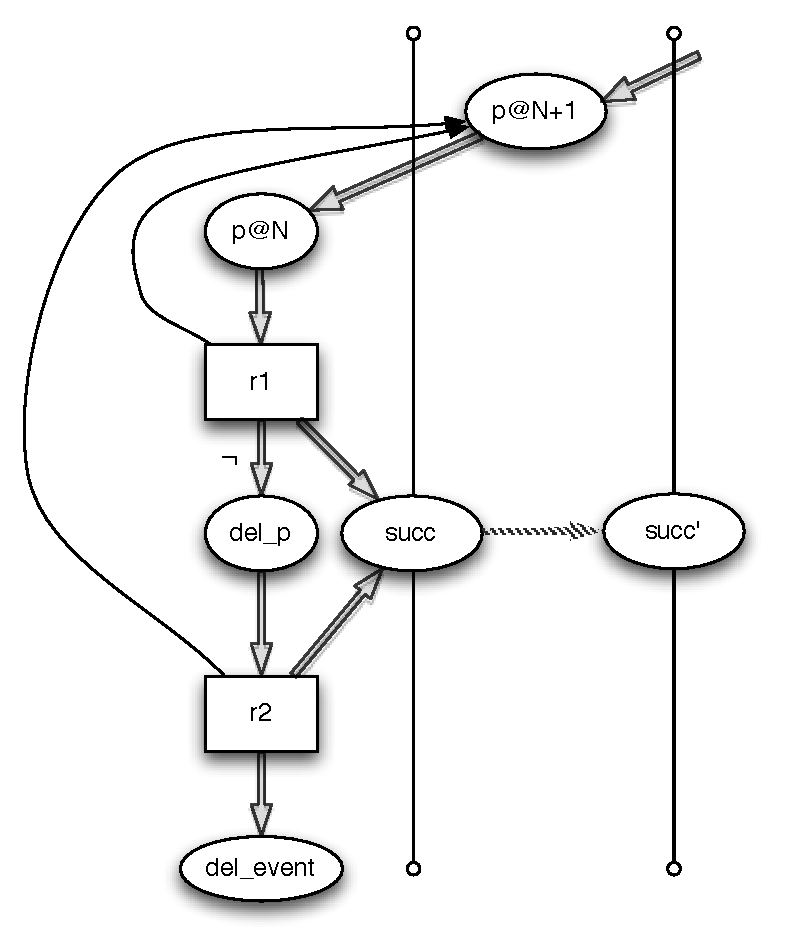
\includegraphics[width=0.5\linewidth]{localstrat_rgg.pdf}
  \label{fig:lstrat}
  \caption{Mutable persistence is locally stratified on time}
\vspace{-8pt}
\end{figure}


\subsubsection{Static Evaluation}
\newtheorem{theorem}{Theorem}

\begin{theorem}
Every Dedalus program P with only deductive rules is equivalent to a Datalog program P'.
\end{theorem}

\begin{proof}
All rules in such a program will be in the form (shown propositionally for simplicity): 

%%\begin{Dedalus}
$p@N \leftarrow b_{1}@N, b_{2}@N, [...], b_{n}@N$
%%\end{Dedalus}

Where p is a head predicate and the $b$s are body predicates.  Note that all time suffixes are 
the same.

Because the time suffix is outside the scope of Datalog, a Datalog fact in the form:

$q(A_{1}, A_{2}, [...], A_{n});$

may be interpreted (equivalently) as persistently true (hence quantified over all logical times $N$) or instantaneously
true at some N.  If we follow the first interpretation, we have 

$q(C_{1}, C_{2}, [...], C_{n})@N;$

The variable N is now universally quantified in the program and in the EDB.  We may eliminate all occurrences of the time suffix N
in rules and facts, and are left with a Datalog program and EDB.

If we follow the second interpretation, the fact is true at some N, so we are given a ground event.  We extend every predicate in 
the program to contain an extra attribute that contains the time suffix value, and move the expression into the predicate as shown below:

$p(A_{1}, A_{2}, [...], A_{n})@N;$\\
$\rightarrow$\\
$p(A_{1}, A_{2}, [...], A_{n}, N);$

The resulting program and EDB are Datalog, and correspond to the intended semantics for the original Dedalus program.

\end{proof}


\subsubsection{Post-hoc Evaluation}

Consider a relation \emph{successor} defined in the following way.
Define first a (2nd order) predicate called \emph{event\_time} 
that contains the union of the time attributes from the EDB of events; i.e.

$event\_time(Time) \leftarrow \displaystyle\bigcup_{i}^n \pi_{Time}EDB_{i}$

\begin{Dedalus}
smax(max<N>) \(\leftarrow\) event\_time(N);
smin(min<N>) \(\leftarrow\) event\_time(N);

successor(N, N + 1) \(\leftarrow\) smin(N);

successor(S, S + 1) \(\leftarrow\) 
    successor(N, S),
    smax(M),
    N <= M;
\end{Dedalus}


\begin{theorem}
Every Dedalus program P with deductive and inductive rules and trace T is equivalent to a Datalog program P' with an EDB T'.
\end{theorem}

\begin{proof}

Extend every predicate to include a final integer attribute as shown in Theorem 1, and drop the body suffixes.  To each rule with an 
inductive head, add the subgoal 

$successor(N, S)$

To each other subgoal, set the new attribute to the variable N.  For the head, set it to S.  Rewrite the event trace in the same fashion, 
moving the event times from the suffix into the final attribute as shown above.


This gives us everything we need to simulate the history of evaluation of the program P using the program P'' and a Datalog interpreter.

\end{proof}

Note, however, that we need arithmetic functions to populate the successor relation.

\begin{theorem}
something about 'for any Dedalus program P and trace T, we may simulate its evaluation with a Datalog program P' and an EDB T'.  this program
will probably not produce side-effects (ie messages) at the same times as the original program, but the evaluation will otherwise be identical.'
\end{theorem}

introduce the $r()$ function, how we can model it using choice, and why it needs the entire successor relation to work properly.



\subsubsection{Continuous Evaluation}

Of course, we are interested in the dynamic and infinite case (\ref{fig:dedalus-time}).
Probably what we want to show is that the IDB database at any timestep of a continuous evaluation is a subset
of the post-hoc interpretation database: specifically, a partition of it on the time attribute.  (unfortunately, presumably
negation in programs can make this not so.)  therefore a constructive interpretation of the infinite sequence of time is permissible:
at each step of computation, we are given ground, a set of rules that tell us what is known now, and a counter value that increments
at each step.  this counter represents the single partition (a single row) of the infinite, totally ordered successor relation.
in some sense, we could argue that this is the only counter construct that needs to be available to the language.

To evaluate programs under the continuous interpretation, we define a special view called \emph{now} which contains the current 
time value.

\begin{Dedalus}
now()@N+1  \(\leftarrow\)
    now()@N;

prev(N)@N+1  \(\leftarrow\)
    now()@N;

panic()  \(\leftarrow\)
    now()@N,
    prev(M),
    M != (N + 1);
\end{Dedalus}

Every rule in a continuous Dedalus program can be considered to be rewritten to include a predicate

$now()@N$

such that $N$ unifies with the time variables in all predicates including \emph{successor}.  This constrains the evaluation of all deductive 
rules to a single partition (really, a single value) of \emph{successor}, and all inductive rules to consider only this and the successor partition.

\subsubsection{Persistence and Stratifiability}


The difficulty with the continuous interpretation is that we must consider the \emph{successor} relation as infinite, which clearly leads
to unsafe programs.  To make matters worse, many useful programs that mutate state will be unstratifiable, because \emph{del\_p} predicate
will be defined negatively in terms of the positive \emph{p} predicate.  For example, take the program below in which \emph{insert\_p}
and \emph{delete\_p} are external events:

\begin{Dedalus}
p(A, B, T)@N+1 \(\leftarrow\)
  p(A, B, T)@N,
  \(\lnot\)del\_p(A, B, T)@N;
  
  
p(A, B, T)@N \(\leftarrow\)
  insert\_p(A, B, T)@N;
  
del_p(A, B, T)@N \(\leftarrow\)
  p(A, B, T)@N,
  delete\_p(T)@N;
\end{Dedalus}

This reasonable program is unstratifiable because $p > del\_p \land del\_p > p$.  

We sidestep these difficulties in two ways:

\begin{enumerate}
\item By joining \emph{now}, we only consider one finite partition (really, one value) of \emph{successor} in a given fixpoint.
\item Any finite partition of \emph{successor}, including any that we may consider in the post-hoc interpretation, is locally stratified. 
\end{enumerate}
